\documentclass[12pt]{exam}
\usepackage{amsmath,amsfonts,amssymb}
\usepackage{diagbox}
\usepackage[colorlinks]{hyperref}
\usepackage{graphicx,caption,subcaption}
\usepackage{tikz}
\usepackage{geometry}
\usepackage{textgreek}
\usepackage[T1]{fontenc}
\geometry{%
  letterpaper,
  lmargin=1.5cm,
  rmargin=1.5cm,
  tmargin=2cm,
  bmargin=2cm,
  footskip=12pt,
  headheight=12pt
}
\usepackage[parfill]{parskip}
\newcommand{\ATAN}{\operatorname{TAN}^{-1}}
\DeclareMathOperator{\COS}{COS}
\usepackage{lastpage}
\headheight 35pt

\lhead{Mathcounts 2020}

\def\a{{\alpha}}
\def\b{{\beta}}
\def\g{{\gamma}}
                   
\DeclareUnicodeCharacter{2212}{-}  

\qformat{}

\begin{document}

\thispagestyle{empty}

\begin{center}\section*{AMC10 2019 A20}

\end{center}
\bigskip
\begin{questions}

\question 
The numbers $1, 2, ..., 9$ are randomly placed into the 9 squares of a $3 x 3$ grid. Each 
square gets one number, and each of the numbers is used once. What is the probability that
the sum of the numbers in each row and each column is odd?
\bigskip

\begin{oneparchoices}
    \choice $\frac{1}{21}$
    \choice $\frac{1}{14}$
    \choice $\frac{5}{63}$
    \choice $\frac{2}{21}$
    \choice $\frac{1}{7}$
\end{oneparchoices}

\vspace{0.5cm}
Odd sums can only be formed in two patterns: $(e, e, o)$ or $(o, o, o)$.
Looking at possible placements of the $e$s, we can find 9 patterns that work:
\begin{itemize}
    \item 4 arranged in a square (4 arrangements, with one square in each corner)
      \\[0.25cm]
      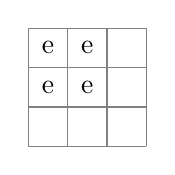
\begin{tikzpicture}
      \draw[step=0.5cm,color=gray] (0.5, -0.5) grid (2, 1);
      \node at (0.75,+0.75) {e};
      \node at (0.75,+0.25) {e};
      \node at (1.25, +0.75) {e};
      \node at (1.25,+0.25) {e};
      \end{tikzpicture}
      
    \item 2 across from 2, with a space in between (4 arrangements)
      \\[0.25cm]
      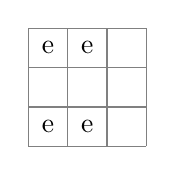
\begin{tikzpicture}
      \draw[step=0.5cm,color=gray] (0.5, -0.5) grid (2, 1);
      \node at (0.75,+0.75) {e};
      \node at (0.75,+-.25) {e};
      \node at (1.25, +0.75) {e};
      \node at (1.25, -.25) {e};
      \end{tikzpicture}
    
    \item 4 in each corner (1 arrangement)
      \\[0.25cm]
      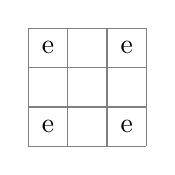
\begin{tikzpicture}
      \draw[step=0.5cm,color=gray] (0.5, -0.5) grid (2, 1);
      \node at (0.75,+0.75) {e};
      \node at (0.75,-0.25) {e};
      \node at (1.75, +0.75) {e};
      \node at (1.75,-0.25) {e};
      \end{tikzpicture}
  
\end{itemize}

\vspace{0.5cm}
Therefore, there are $9 \times 4! \times 5!$ arrangements that 
satisfy the conditions. The probability is $\frac{9 \times 4! \times 5!}{9!}$, 
which is $\frac{1}{14}$. B $\left (\frac{1}{14} \right)$.

\end{questions}
\end{document}